\problemname{Astronoms}

\illustration{.3}{img/TychoBrahe.JPG}{}

\noindent
Astronomam ir aizraušanās vērot zvaigznes.
Konkrētāk, viņš izjūt neaprakstāmu prieku vienlaikus vērojot $k$ zvaigznes caur savu teleskopu.
Teleskopa ar rādiusu $r$ izveide maksās $t\cdot r$ kronas.
Jauns teleskops būs vērsts tieši uz sākumpunktu $(0,0)$.
Tā pavēršana uz citu punktu debesīs rada papildus izmaksas;
pavēršot teleskopu uz citu punktu debesīs attālumā $d$ vienības izmaksā $s\cdot d$ kronas.
Astronoms var novērot visas zvaigznes, kas atrodas attālumā ne vairāk kā $r$ no punkta, uz kuru ir pavērsts teleskops.

Cik maksās izveidot un pavērst teleskopu, lai varētu novērot $k$ zvaigznes vienlaikus?

\medskip

Visas koordinātas un attālumi ir doti Eiklīda plaknē.

\section*{Piemērs}

Lūk, piemērs ar $n=3$ zvaigznēm, kuru koordinātas ir $(0,0)$, $(2,0)$ un $(3,1)$.
Iekrāsotais laukums reprezentē teleskopu ar rādiusu 1, kas ir pavērsts uz koordināti (1, 0) un
tajā vērojamas divas zvaigznes. Tas izmaksā $s + t$~kronas un ir optimāls risinājums $3$. parauga ievaddatiem.
Attēls arī parāda optimālos risinājumus $1.$, $2.$ un $4.$ parauga ievaddatiem.

\medskip
\noindent
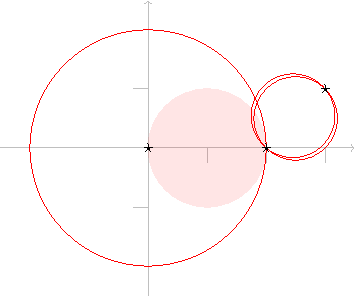
\includegraphics[width=.3\textwidth]{img/samples.pdf}

\section*{Ievaddati}

Pirmā rindiņa satur četrus veselus skaitļus:
zvaigžņu skaitu $k$, ko astronoms vēlas novērot,
zvaigžņu skaitu šīs nakts debesīs $n$,
izmaksas $s$ par teleskopa pārvietošanu un
izmaksas $t$ par teleskopa būvniecību.
Tad seko $n$ rindas, kur $i$-tajā rindā ir $i$-tās zvaigznes koordinātes $(x_i,y_i)$.

\section*{Izvaddati}

Viens reāls skaitlis: vismazākais izdevumu apjoms kronās, kas astronomam jāiztērē.

\section*{Ierobežojumi un vērtēšana}

Var pieņemt, ka
\begin{enumerate}
\item $1\leq k\leq n\leq 700$. % constraint:kn
\item $x_i, y_i\in \{-10^9,\ldots, 10^9\}$ visiem $i\in\{1,\ldots,n\}$. % constraint:xy
\item $s,t\in \{0,\ldots, 10^9\}$. % constraint:st
\item Jūsu atbilde tiek uzskatīta par pareizu, ja tās absolūtā vai relatīvā kļūda ir $\epsilon = 10^{-6}$ robežās.
\end{enumerate}

Jūsu risinājums tiks pārbaudīts uz vairākām testu grupām. Katra grupa ir vērta noteiktu punktu skaitu.
Katra testu grupa satur vairākus testus.
Lai saņemtu punktus par testu grupu, ir jāatrisina visi testi testu grupā.
Jūsu gala rezultāts būs lielākais punktu skaits, kas iegūts ar vienu risinājuma iesniegumu.

\medskip
\noindent
\begin{tabular}{lll}
  Grupa & Punkti & Ierobežojumi\\\hline
  $1$ & $8$ &  $t\leq s$\\
  $2$ & $9$ & $n\le 50$ un $s=0$\\
  $3$ & $18$ & $s=0$\\
  $4$ & $13$ & $n\leq 50$\\
  $5$ & $14$ & $n\leq 350$\\
  $6$ & $15$ & $\epsilon = 1/10$\\
  $7$ & $23$ & \emph{Bez papildu ierobežojumiem}\\
\end{tabular}
